
%(BEGIN_QUESTION)
% Copyright 2014, Tony R. Kuphaldt, released under the Creative Commons Attribution License (v 1.0)
% This means you may do almost anything with this work of mine, so long as you give me proper credit

Calculate the current through the ``B'' line given the phase voltages and load inductance/resistance values shown, assuming a system frequency of 60 Hz:

$$\includegraphics[width=15.5cm]{i03123x01.eps}$$

$V_A$ = 2.4 kV $\angle$ 0$^{o}$ \hskip 20pt $V_B$ = 2.4 kV $\angle$ $240^{o}$ \hskip 20pt $V_C$ = 2.4 kV $\angle$ $120^{o}$

\vskip 10pt

Your answer needs to specify both the magnitude of $I_B$ as well as its phase angle:

\vskip 10pt

$I_B$ = \underbar{\hskip 80pt} 

\underbar{file i03123}
%(END_QUESTION)





%(BEGIN_ANSWER)

$I_B$ = 1.993 A $\angle$ $188.5^o$ \hskip 10pt or \hskip 10pt 1.993 A $\angle$ $-171.5^o$  
 
%(END_ANSWER)





%(BEGIN_NOTES)

{\bf This question is intended for exams only and not worksheets!}.

%(END_NOTES)


